\section{Algorithme d'apprentissage}
\label{sec:kernel}

\epigraph{The word “algorithm” itself is quite interesting; at first glance it may look as
  though someone intended to write “logarithm” but jumbled up the first four
  letters.}{Donald Knuth\\\textsc{The Art of Computer Programming, Volume I}}


Cette section sera l'occasion d'étudier l'algorithme $\alg:M^n \to \Q$ permettant d'obtenir
une politique d'investissement empirique $\qh$ à partir d'un ensemble d'entraînement
$\S_n = \{(r_1,x_1),\ldots,(r_n,x_n)\}$ échantilloné de la loi de marché $M$.

Les formulations primale et duale seront d'abord présentées dans le cas où l'espace des
variables de marché $\X$ ne subit aucune transformation. Ces deux formulations seront
ensuite généralisées au cas non linéaire obtenu par application $x \mapsto \phi(x)$. Finalement
l'``astuce du noyau'', qui permet de représenter des situations complexes où $\phi(x)$ est
possiblement de dimension infinie, sera introduite. 


\subsection{Formulations primale et duale}

Tel que discuté en introduction, les décisions d'investissement considérées dans ce
mémoire seront données par produit scalaire. Le cas le plus simple pour un espace de
décision est alors celui où l'espace $\X$ des variables de marché ne subit aucune
transformation. L'espace $\Q$ correspond\footnote{En fait, pour être exact,
  $q : \X \to \Re$ étant une \textit{fonction}, il est plus exact de faire correspondre
  $\Q$ à l'espace \textit{dual} $\X^*$. Mais par le théorème de Riez, à tout vecteur
  $v \in \bm V$ d'un espace vectoriel, il existe un unique vecteur dual $v^* \in \bm V^*$
  (noté $v^T$ en dimension finie). On peut donc se contenter de faire correspondre $\Q$ à
  $\X$.}\footnote{Ici aussi on fait une approximation: $\Q$ ne correspond pas
  nécessairement à $\X$, mais bien à $\Re^p$ où $p = \dim\X$. En effet, $\X$ représente le
  support du vecteur aléatoire de marché et est possiblement borné, alors qu'on ne veut
  pas imposer une telle restriction à $\Q$. Cependant la notation demeure plus claire
  ainsi. } alors à $\X$ et le scalaire de décision $q(x)$ est obtenu par produit scalaire
$q^Tx$. On obtient donc ici le problème sous la forme \textit{primale}: {\begin{equation}
    \boxed{ \maximizeEquation[q\in\X]{n^{-1}\sumi u(r_i\,q^Tx_i) - \frac{\lambda}{2}\|q\|^2}}
\end{equation}
\vspace{-\baselineskip}\captionof*{figure}{\textit{Formulation primale I}}}

Par la théorie de l'optimisation convexe (voir par exemple le Lemme 6 de
\cite{nesterov2009primal}) on sait qu'une solution $\qh$ existe et qu'elle est unique. En
supposant que $p = \dim\X$, on peut alors exprimer $\qh$ comme une combinaison de $p$
coordonnées.

Cependant, $\qh$ peut aussi être exprimé comme une combinaison linéaires des $n$
observations $\{x_1,\ldots,x_n\}$. Autrement dit, il existe un vecteur
$\hat\alpha \in \Re^n$ tel que $\qh = \Xi^T\hat\alpha$, où $\Xi \in \Re^{n \times p}$ est la matrice des
observations.

Il suffit en effet de remarquer que l'espace $\Q = \X$ peut être décomposé comme la somme
directe du sous-espace vectoriel $\hat\X$ engendré par $\Xi^T$ et son complément orthogonal
$\hat\X^\perp$, \ie\ $\Q = \hat\X \oplus \hat\X^\perp$. Ainsi, tout vecteur de décision
$q \in \Q$ s'exprime comme la somme de $\hat x\in\hat\X$ et
$\hat x^\perp \in \hat\X^\perp$, deux vecteurs orthogonaux (voir les appendices de
\cite{boyd2004convex} ou \cite{mohri2012foundations}). La fonction objectif $\EU_\lambda$
évaluée au point $q = \hat x + \hat x^\perp$ choisi arbitrairement se simplifie alors ainsi:
\begin{align}
  \EU_\lambda(q) &= \EU_\lambda(\hat x + \hat x^\perp)\\
           &= n^{-1}\sumi u(r_i\,(\hat x + \hat x^\perp)^Tx_i) - \frac{\lambda}{2}\|\hat x + \hat
             x^\perp\|^2\\
           &\leq n^{-1}\sumi u(r_i\,\hat x^Tx_i) - \frac{\lambda}{2}\|\hat x\|^2\\
           &=\EU_\lambda(\hat x),
\end{align}
puisque, par définition, $(\hat x^\perp)^Tx_i = 0$ pour toute observation $x_i$ et que d'autre
part $\|\hat x\|^2 \leq \|\hat x\|^2+\|\hat x^\perp\|^2 = \|q\|^2$. Ainsi, toute solution
$\qh$ repose bien dans l'espace colonne de $\Xi^T$.

Cette observation (qui correspond en fait au célèbre théorème de la représentation: voir
\cite{scholkopf2001learning} pour un traitement rigoureux de l'apprentissage par noyau)
peut se révéler très utile car elle permet de changer le domaine d'optimisation de $\X$ à
$\Re^n$ par l'identité $\qh = \Xi^T\hat\alpha$. Autrement dit, le problème d'optimisation devient
\begin{equation}
  \maximizeEquation[\alpha \in \Re^n]{n^{-1}\sumi u(r_i\,\alpha^T\Xi x_i) - \frac{\lambda}{2}\alpha^T\Xi\Xi^T\alpha.}
\end{equation}
On peut simplifier cette expression en posant $K \coloneqq \Xi\Xi^T \in \Re^{n \times n}$:
{\begin{equation}
  \boxed{
  \maximizeEquation[\alpha \in \Re^n]{n^{-1}\sumi u(r_iK_i\alpha) - \frac{\lambda}{2}\alpha^TK\alpha,}}
\end{equation}
\vspace{-\baselineskip}\captionof*{figure}{\textit{Formulation duale I}}}
où $\sum_{j=1}^nx_j^Tx_i = K_i \in \Re^n$ représente la $i$\ieme colonne (ou rangée car
$K$ est alors symétrique) de $K$. En fait $K$ correspond à la \textit{matrice gramienne},
\ie\ la matrice des produits scalaires de toutes les observations $x_i$.

On peut par ailleurs remarquer que ce résultat était déjà annoncé par le cas spécial où
l'utilité de l'investisseur est risque neutre. On a souligné en introduction que dans un
tel cas, la solution optimale pouvait effectivement s'exprimer comme une moyenne pondérée
des $n$ observations (voir aussi le Lemme \ref{lem:ndef} en Appendice \ref{sec:lems}):
\begin{equation}
  \qh = \frac{1}{n\lambda}\sumi r_i x_i
\end{equation}
et on obtient donc $\hat\alpha = (n\lambda)^{-1}r$. 



\subsection{Transformations non linéaires}

Le cas $\Q = \X$ est cependant trop simple pour rendre compte de certaines géométries de
problème. En fait, certaines géométries du problème peuvent donner lieu à des situations
où aucune solution n'est vraiment satisfaisante. Par exemple, le panneau a) de la Figure
\ref{fig_xor} présenterait à l'investisseur un dilemme de taille puisqu'aucune fonction de
décision affine ne permet d'attribuer un investissement positif aux rendements positifs ou
un investissement négatif aux rendements négatifs. Il s'agit du problème XOR bien connu en
apprentissage machine.


\begin{figure}[p]
  \centering
  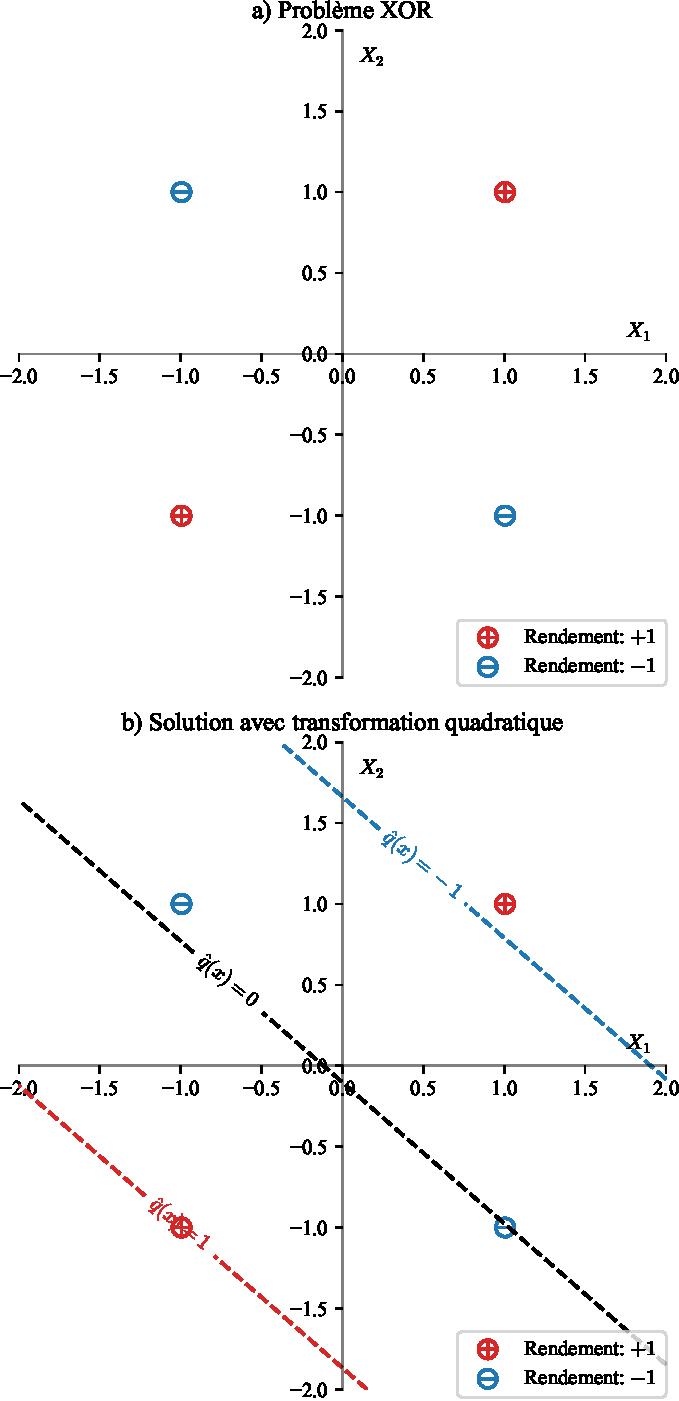
\includegraphics[width=0.65\textwidth]{../experiments/fig/pres/pres5_fr.pdf}
  \caption[Problème XOR]{Ensemble d'entraînement XOR. Au paneau a), aucune décision
    linéaire ne permet d'attribuer à des rendements positifs une décision d'investissement
    positive, et de la même façon pour les rendements positifs. Le panneau b) présente la
    solution optimale avec transformation quadratique lorsque $u(r)=-e^{-r}+1$ et
    $\lambda=0.1$.}
  \label{fig_xor}
\end{figure}


Il est alors naturel de définir une transformation non linéaire de l'espace $\X$ par une
fonction $\phi:\X\to\phi(\X)$. Par exemple, si $\X \in \Re$, \ie\ une seule variable de marché n'est
considérée, alors on peut chercher une solution polynômiale en posant la transformation
suivante:
\begin{equation}
  \phi:x \mapsto
  \begin{pmatrix}
    1 \\ x \\ x^2 \\ \vdots \\ x^k
  \end{pmatrix}.
\end{equation}
Cette transformation se généralise en plusieurs dimensions en considérant aussi les termes
croisés.

En notant $\inp{\cdot,\cdot}$ le produit scalaire de l'espace $\phi(\X)$, le problème consiste alors
à trouver un vecteur optimal $q \in \Q = \phi(\X)$ de façon à
{\begin{equation}
    \boxed{
      \maximizeEquation[q\in\phi(\X)]{n^{-1}\sumi u(r_i\,\inp{q,\phi(x_i)}) - \frac{\lambda}{2}\|q\|^2.}}
  \end{equation}
  \vspace{-\baselineskip}\captionof*{figure}{\textit{Formulation primale II}}}

Mais puisque le théorème de représentation s'applique encore, $\qh$ peut aussi s'exprimer
comme une combinaison linéaire $\alpha$ des observations $\{\phi(x_1) ,\ldots, \phi(x_n)\}$:
{\begin{equation}
\boxed{
  \maximizeEquation[\alpha \in \Re^n]{n^{-1}\sumi u(r_iK_i\alpha) - \frac{\lambda}{2}\alpha^TK\alpha.}}
\end{equation}
\vspace{-\baselineskip}\captionof*{figure}{\textit{Formulation duale II}}}
Cette fois par contre $K_{ij} = \inp{\phi(x_i),\phi(x_j)}$; chaque élément de $K$ représente le
produit scalaire des éléments $\phi(x_i)$. Une fois qu'une solution $\hat\alpha$ est obtenue, la
décision optimale est donnée par $\qh(x) = \sumi \alpha_i\langle\phi(x_i),\phi(x)\rangle$. 

Le panneau b) de la Figure \ref{fig_xor} illustre comment une transformation quadratique
permet de résoudre le problème XOR.


\subsection{Fonctions de noyau}

Ainsi, pour toute transformation $\phi:\X\to\phi(\X)$, quelle que soit la dimension de l'espace
$\phi(\X)$, on peut exprimer la décision optimale à partir d'une optimisation sur $n$
dimensions. En outre, ce programme d'optimisation ne dépend plus que du produit scalaire
entre ces observations transformées. De plus, on peut dans bien des cas court-circuiter le
calcul de ce produit scalaire par une fonction \textit{noyau} $\kappa:\X\times\X \to \Re$ telle que
$\kappa(x_i,x_j) = \inp{\phi(x_i),\phi(x_j)}$.

Par exemple, dans l'exemple à une dimension discuté plus haut, il suffirait de poser
\begin{equation}
  \kappa(x_i,x_j) = 1 + x_ix_j + (x_ix_j)^2 + \cdots + (x_ix_j)^k.
\end{equation}
Évidemment, dans un pareil cas le gain est assez faible puisqu'on a uniquement réarrangé
l'ordre des opérations. Mais, il est alors possible de circonvenir complètement la
transformation $\phi$ et de ne représenter sa non linéarité qu'à partir de $\kappa$. Par exemple,
le noyau gaussien
\begin{equation}
  \kappa(x_i,x_j) = \exp\left(-\frac{\|x_i-x_j\|^2}{2\sigma^2}\right)
\end{equation}
permet de calculer directement le produit scalaire $\inp{\phi(x_i),\phi(x_j)}$ d'observations
$\phi(x_i)$ et $\phi(x_j)$ de dimension infinie
(\cite{mohri2012foundations,scholkopf2001learning}).

Choisir adéquatement le noyau est alors une tâche cruciale du modèle puisque tout noyau
$\kappa$ induit une géométrie particulière du modèle; il peut alors être impossible de
déterminer une fonction de décision $q$ pourvue de bonne performance si le noyau ne
correspond pas à la géométrie de la loi de marché $M$.

Il faut par ailleurs imposer une contrainte supplémentaire à la classe des noyaux
possibles. En effet $\kappa(x_i,x_j)$ représente un produit scalaire dans $\phi(\X)$ et est donc
tenu de respecter les popriétés algébriques de celui-ci. Notamment, $\kappa$ doit satisfaire
l'inégalité de Cauchy-Schwartz:
\begin{align}
  \kappa(x_i,x_j)^2 &= \inp{\phi(x_i),\phi(x_j)}^2\\
               &\leq \|\phi(x_i)\|\|\phi(x_j)\|\\
               &= \kappa(x_i,x_i)\kappa(x_j,x_j).
\end{align}
Mais plus précisément, le noyau $\kappa$ doit être une forme symétrique bilinéaire définie
positive sur $\X$ (voir encore \cite{mohri2012foundations,scholkopf2001learning}).




\subsection{Espace de décision vectoriel}


Enfin, cette fonction noyau est également en mesure \textit{d'induire} un espace de
décision par la relation $\Q = \kappa(\X,\cdot)$. L'espace de décision ainsi obtenu est alors un
\textit{espace de Hilbert à noyau reproduisant}, et donc un espace vectoriel. Autrement
dit, les opérations comme la norme, l'addition ou le produit scalaire sont supportés et
peuvent être appliquées sur des fonctions de décision $q \in \Q$. Dans le cas linéaire, on
revient au cas où $\Q$ correspond au dual de $\X$. 

On peut de surcroît introduire une nouvelle notation qui offre une symétrie avec le cas
linéaire. En notant
\begin{align}
  |\cdot\rangle&:\X \to \Q \\ 
|x\rangle &\coloneq \kappa(x,\cdot)
\end{align}
la transformation d'un point $x\in\X$ vers sa fonction dans $\Q$ et  
\begin{align}
  \langle\cdot|&:\Q \to \Q^*\\
  \langle q| &\coloneq q^*
\end{align}
l'élément dual d'un élément de $\Q$, on peut obtenir l'identité
\begin{equation}
  q(x) = \langle q|x \rangle,
\end{equation}
c'est à dire le produit scalaire entre $q$ et $|x\rangle$. Par exemple, on peut alors exprimer
la solution du problème à utilité neutre au risque simplement comme
\begin{equation}
  \qh = \frac{1}{n\lambda}\sumi r_i|x_i\rangle,
\end{equation}
quel que soit le noyau ou la transformation employé.


\subsection{Conclusion}

La méthode des noyaux, qui permet de généraliser toute transformation non linéaire $\phi$,
est d'une importance capitale dans ce travail puisqu'elle rend compte de situations
complexes, tout en conservant les avantages offerts par un algorithme de maximisation
d'utilité espérée convexe qui seront présentés à la section suivante.

Enfin, la Figure \ref{fig_yeah} offre à titre d'exemple les solutions quadratiques et
gaussiennes obtenues sur l'ensemble d'entraînement fictif de la Figure
\ref{fig_pres1}. Notamment, bien que la transformation quadratique du panneau a) ne soit
toujours pas en mesure de suggérer un investissement cohérent avec toutes les
observations, on constate cependant que la transformation gaussienne b) y parvient sans
problème.

\begin{figure}[p]
  \centering
  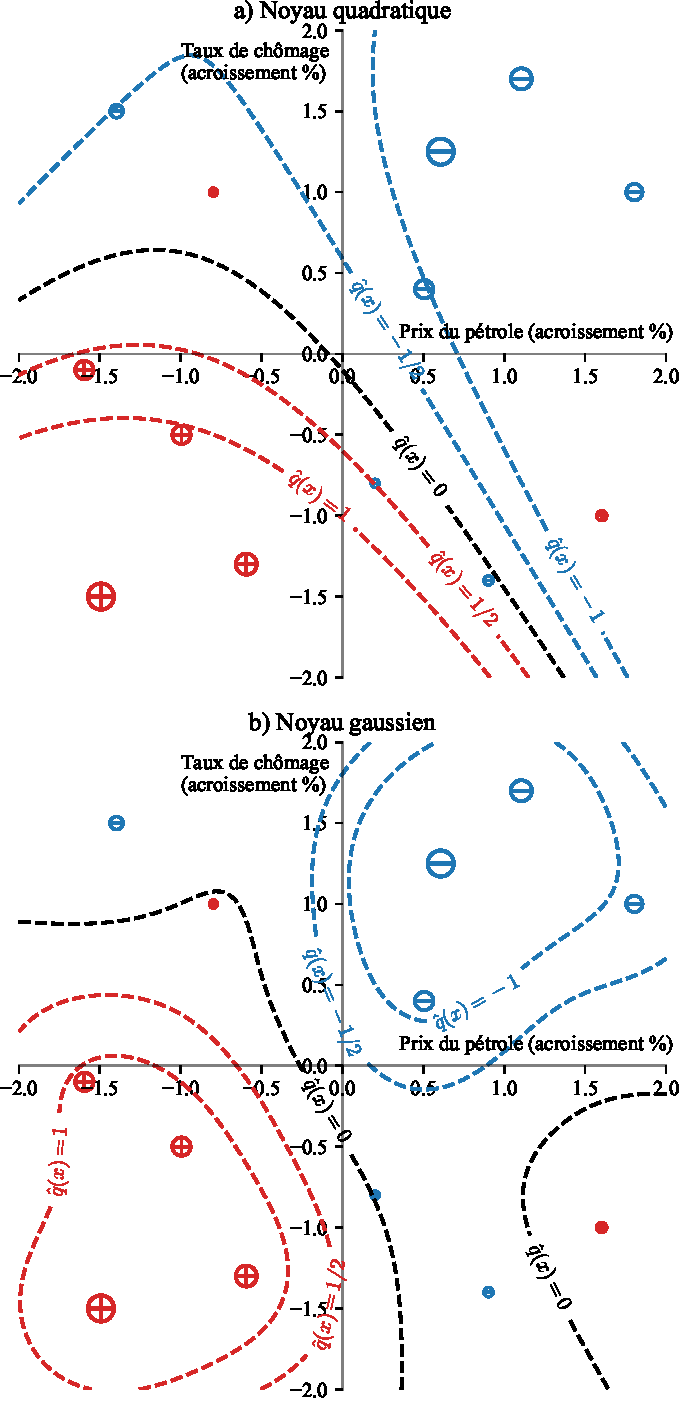
\includegraphics[width=0.65\textwidth]{../experiments/fig/pres/pres10_fr.pdf}
  \caption[Solutions quadratique et gaussienne]{Deux solutions au problème de la Figure
    \ref{fig_pres1}. En utilisant un noyau quadratique (panneau a)), on obtient une plus
    grande complexité, mais certains points demeurent mal ``classés''. Par contre, au
    panneau b), le noyau gaussien offre une flexiblité suffisante pour bien classer toutes
    les observations. Dans les deux cas, une utilité de $u(r) = -e^{-r}+1$ et une
    régularisation $\lambda=0.1$ ont été employés. Le noyau gaussien a une bande passante
    $\sigma = 1/2$. }
  \label{fig_yeah}
\end{figure}









%%% Local Variables:
%%% mode: latex
%%% TeX-master: "memoire"
%%% End:
